
\section{Matrixfunktionen}

Matrixfunktionen bieten uns die Möglichkeit, nach bestimmten Kriterien Werte aus Listen oder Bereichen zu entnehmen, ihre Positionen zu bestimmen oder bieten uns Hilfestellungen dafür an. 


\subsection{\stmt{VERGLEICH}}

$$ \text{\stmt{   VERGLEICH(\syntax{Suchkriterium}; \syntax{Suchmatrix}; [\syntax{Vergleichstyp}])  }}$$

Die \stmt{VERGLEICH} Funktion wird dann verwendet, wenn man nicht den Wert aus einer Spalte oder Zeile haben will, sondern die Position bezogen auf die Suchmatrix.


\begin{description}[labelindent=0cm, leftmargin=3cm, font=\mdseries, labelwidth=3cm,style=nextline]
\item[\syntax{Suchkriterium}] Wert nach dem in der \syntax{Suchmatrix} gesucht werden soll
\item[\syntax{Suchmatrix}] ist entweder ein Zeilenbereich, z.B. \stmt{\upquote{A2:H2}}, oder ein Spaltenbereich, z.B. \stmt{\upquote{A2:A6}}, in dem gesucht werden soll.
\item[\syntax{Vergleichstyp}] %
	\begin{description}[labelindent=0cm, leftmargin=2cm, font=\mdseries, labelwidth=2cm,style=nextline]
	\item[1 (default)] Sucht nach dem größtem Wert, der kleiner oder gleich dem Suchkriterium ist. Die Suchmatrix muss daher zwingend \textsl{aufsteigend} sortiert sein.
	\item[0] Sucht exakt das Suchkriterium in der Suchmatrix. Das Suchkriterium muss in
der Suchmatrix vorkommen, die Suchmatrix muss aber nicht sortiert sein.
	\item[-1] Sucht nach dem kleinsten Wert, der größer oder gleich dem Suchkriterium ist.
Die Suchmatrix muss daher zwingend \textsl{absteigend} sortiert sein.
	\end{description}

\end{description}

Im folgenden Beispiel ist das Suchkriterium der Wert 245. \stmt{VERGLEICH} sucht nun im angegebenen Suchbereich jene Zeile, in der der gesuchte Wert größer gleich dem Wert in der Zeile, aber kleiner als der Wert in der nächsten Zeile ist. In diesem Falle, ist es hier die Zeile mit dem Wert 200. Der ist ja kleiner als unser gesuchter Wert. Und der Wert in der nächsten Zeile ist schon größer als unser gesuchter Wert. Der gesuchte Wert ist also in der zweiten Zeile des Suchbereiches und daher liefert die Formel den Wert 2.

	\begin{figure}[H]
		\centering
%			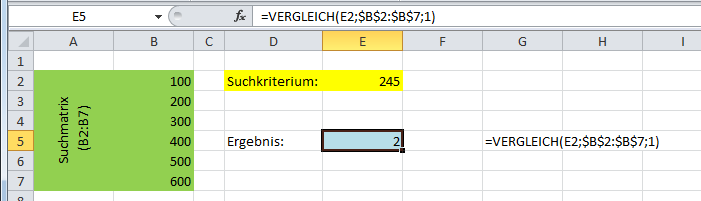
\includegraphics[width=16cm]{images/vergleich_1b}
			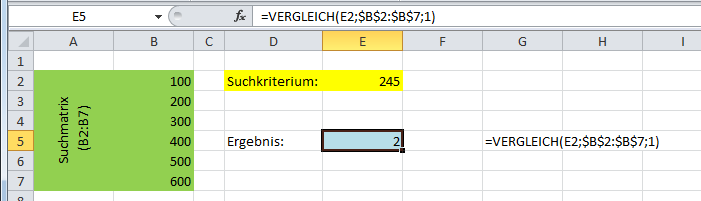
\includegraphics[scale=0.7]{images/vergleich_1b}
		\caption{\stmt{VERGLEICH} in einem Beispiel}
		\label{fig:vergleich_1}
	\end{figure}
	
	
\begin{infobox}%
Wenn der Suchwert kleiner als der kleinste Wert in der Suchmatrix ist, dann wird ein Fehler \stmt{\#NV} retourniert. Fehler wie \stmt{\#NV}, \stmt{\#Wert!}, \stmt{\#Bezug!}, \stmt{\#Div/0!}, \stmt{\#Num!}, \stmt{\#Name!} oder \stmt{\#Null!} können mit der Funktion \stmt{WENNFEHLER(\syntax{Wert}; \syntax{Wert falls Fehler})} abgefangen werden.
\end{infobox}

	\begin{figure}[H]
		\centering
%			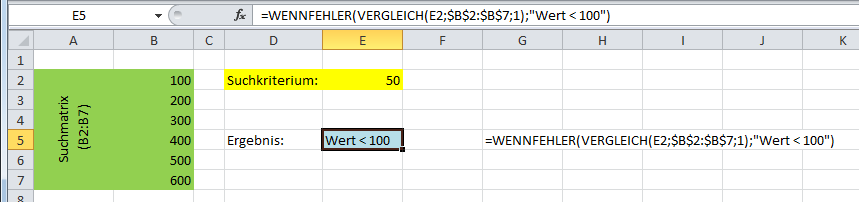
\includegraphics[width=16cm]{images/vergleich_2b}
			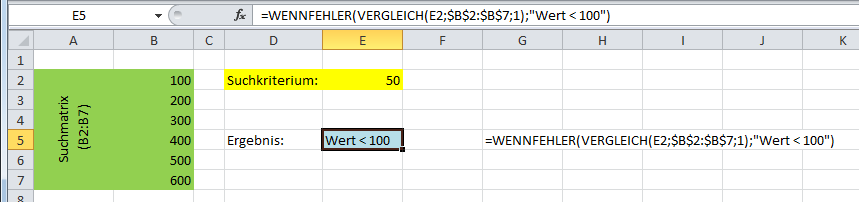
\includegraphics[scale=0.7]{images/vergleich_2b}
		\caption{\stmt{VERGLEICH} mit fehlerhaftem Wert}
		\label{fig:vergleich_fehler}
	\end{figure}

\subsection{\stmt{INDEX} (Matrixversion)}

$$ \text{ \stmt{INDEX( \syntax{Matrix}; \syntax{Zeile}; \syntax{Spalte})}}$$

Die \stmt{INDEX} Funktion liefert aus einer Matrix genau jenen Wert, der im angegebenen Schnittpunkt einer Zeile und einer Spalte steht. Besteht die Matrix aus nur einem Zeilenbereich oder einem Spaltenbereich kann das Argument der Zeile bzw. Spalte weggelassen werden. 
%
Im einfachsten Anwendungsfall, der sehr selten vorkommt, weiß man, in welcher Zeile der Matrix der gewünschte Spaltenwert zu suchen ist. In der \figref{fig:matrix}  wird der Preis der Zitrone gewünscht, welche in der dritten Zeile der Matrix steht.
	\begin{figure}[H]
		\centering
%			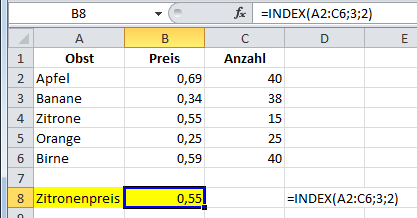
\includegraphics[width=8cm]{images/matrix_1b}
			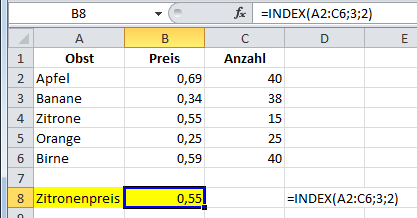
\includegraphics[scale=0.7]{images/matrix_1b}
		\caption{\stmt{MATRIX} Funktion}
		\label{fig:matrix}
	\end{figure}
%
Normalerweise kennt man entweder die Spalte nicht, die Zeile nicht oder auch beides gemeinsam nicht. Wenn das obige Beispiel derart erweitert wird, dass auch die Obstsorte wählbar ist, dann würde die Formel folgendermaßen aussehen.
%
	\begin{figure}[H]
		\centering
%			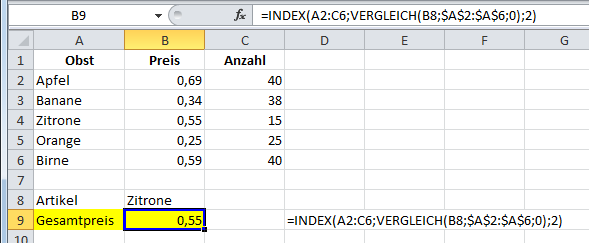
\includegraphics[width=12cm]{images/matrix_mit_vergleich_b}
			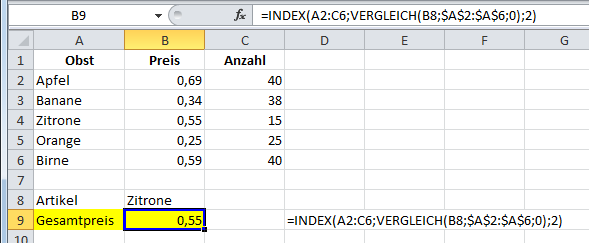
\includegraphics[scale=0.7]{images/matrix_mit_vergleich_b}
		\caption{\stmt{MATRIX} Funktion mit \stmt{VERGLEICH}}
		\label{fig:matrix_mit_vergleich}
	\end{figure}
%
\begin{infobox}%
Es ist wichtig, dass man eventuelle Spalten- oder Zeilenbeschriftungen \textit{nicht} zum Matrixbereich hinzuzählt. Der Matrixbereich ist nur der Wertebereich.
\end{infobox}

\subsection{\stmt{INDEX} (Bezugsversion)}

$$ \text{\stmt{INDEX( \syntax{Matrix}; \syntax{Zeile}; \syntax{Spalte}; [\syntax{Bereich}] )}}$$


Liefert den Bezug jener Zelle, auf die sich Zeile und Spalte in dem angegebenen Bezug (=Zellbereich) beziehen. Für den Paramater \syntax{Bezug} können auch mehrere, voneinander unabhängige Zellbereiche durch \stmt{()} eingeschlossen, angegeben werden.

\begin{description}[labelindent=0cm, leftmargin=3cm, font=\mdseries, labelwidth=3cm,style=nextline]
\item[Bereich]Falls mehrere Bezüge angegeben werden, bezieht sich die Bereichsnummer beginnend mit 1, dem Defaultwert, auf den jeweiligen Bezugsbereich.
\end{description}
%
	\begin{figure}[H]
		\centering
%			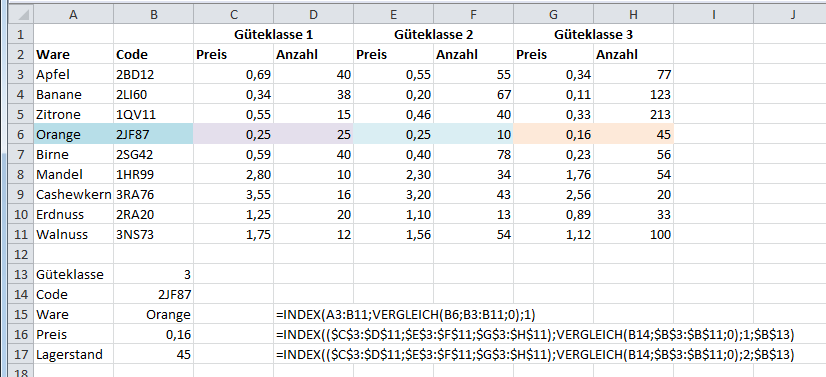
\includegraphics[width=16cm]{images/index_mit_bezug_b}
			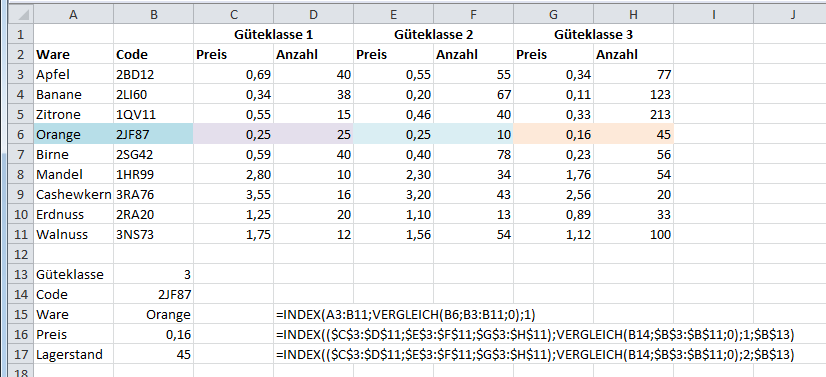
\includegraphics[scale=0.7]{images/index_mit_bezug_b}
		\caption{\stmt{INDEX} Funktion mit mehreren Bereichen}
		\label{fig:matrix_mit_bezug}
	\end{figure}
%
Schauen wir uns die Formel für den Lagerstand in Zelle \xlc{B17} näher an und teilen die einzelnen Parameter zur näheren Erklärung in ihre Einzelteile auf%
$$ \text{ \stmt{=INDEX((\$C\$3:\$D\$11;\$E\$3:\$F\$11;\$G\$3:\$H\$11);VERGLEICH(B14;\$B\$3:\$B\$11;0);2;\$B\$13)} }$$

\begin{description}[labelindent=0cm, leftmargin=8cm, font=\mdseries, labelwidth=8cm,style=nextline]
\item[\stmt{(\$C\$3:\$D\$11;\$E\$3:\$F\$11;\$G\$3:\$H\$11)}]Der erste Parameter umfasst die drei verschiedenen Bereiche mit Preis und Lagerstand.
\item[\stmt{VERGLEICH(B14;\$B\$3:\$B\$11;0)}] Danach wird über die \stmt{VERGLEICH} Funktion die Zeile ermittelt, welche den gewünschten Wert enthält. Ind diesem Fall wird nach dem Code, welcher in \stmt{B14} angegeben ist, im Bereich \stmt{\$B\$3:\$B\$11} gesucht. Und das auf genaue Übereinstimmung.
\item[\stmt{2}] Da der Lagerstand gewünscht ist, soll aus der Matrix der Wert der zweiten Spalte zurückgegeben werden.
\item[\stmt{\$B\$13}] Im letzten Parameter wird nun bestimmt, aus welchem der im ersten Parameter angegebenen Bereiche der Wert genommen wird. Im obigen Beispiel bezeichnet die 3 der Güteklasse auch den dritten Bereich
\end{description}
	
\begin{infobox}%
Es ist absolut wichtig, dass mehrere Bereiche immer durch Klammern \stmt{()} umgeben sind, da sonst ein Fehler ausgegeben wird.
\end{infobox}

\subsection{Beispiel zu \stmt{INDEX} und \stmt{VERGLEICH}}

Die beiden Excel Funktionen \stmt{INDEX} und \stmt{VERGLEICH} arbeiten sehr oft zusammen und daher werden sie hier gemeinsam anhand eines Beispieles eines Obsthändlers erklärt, der wissen will wieviele Melonen im März verkauft wurden.

%\placefigure[middle,force]{}{\externalfigure[indexxls]}
	\begin{figure}[H]
		\centering
%			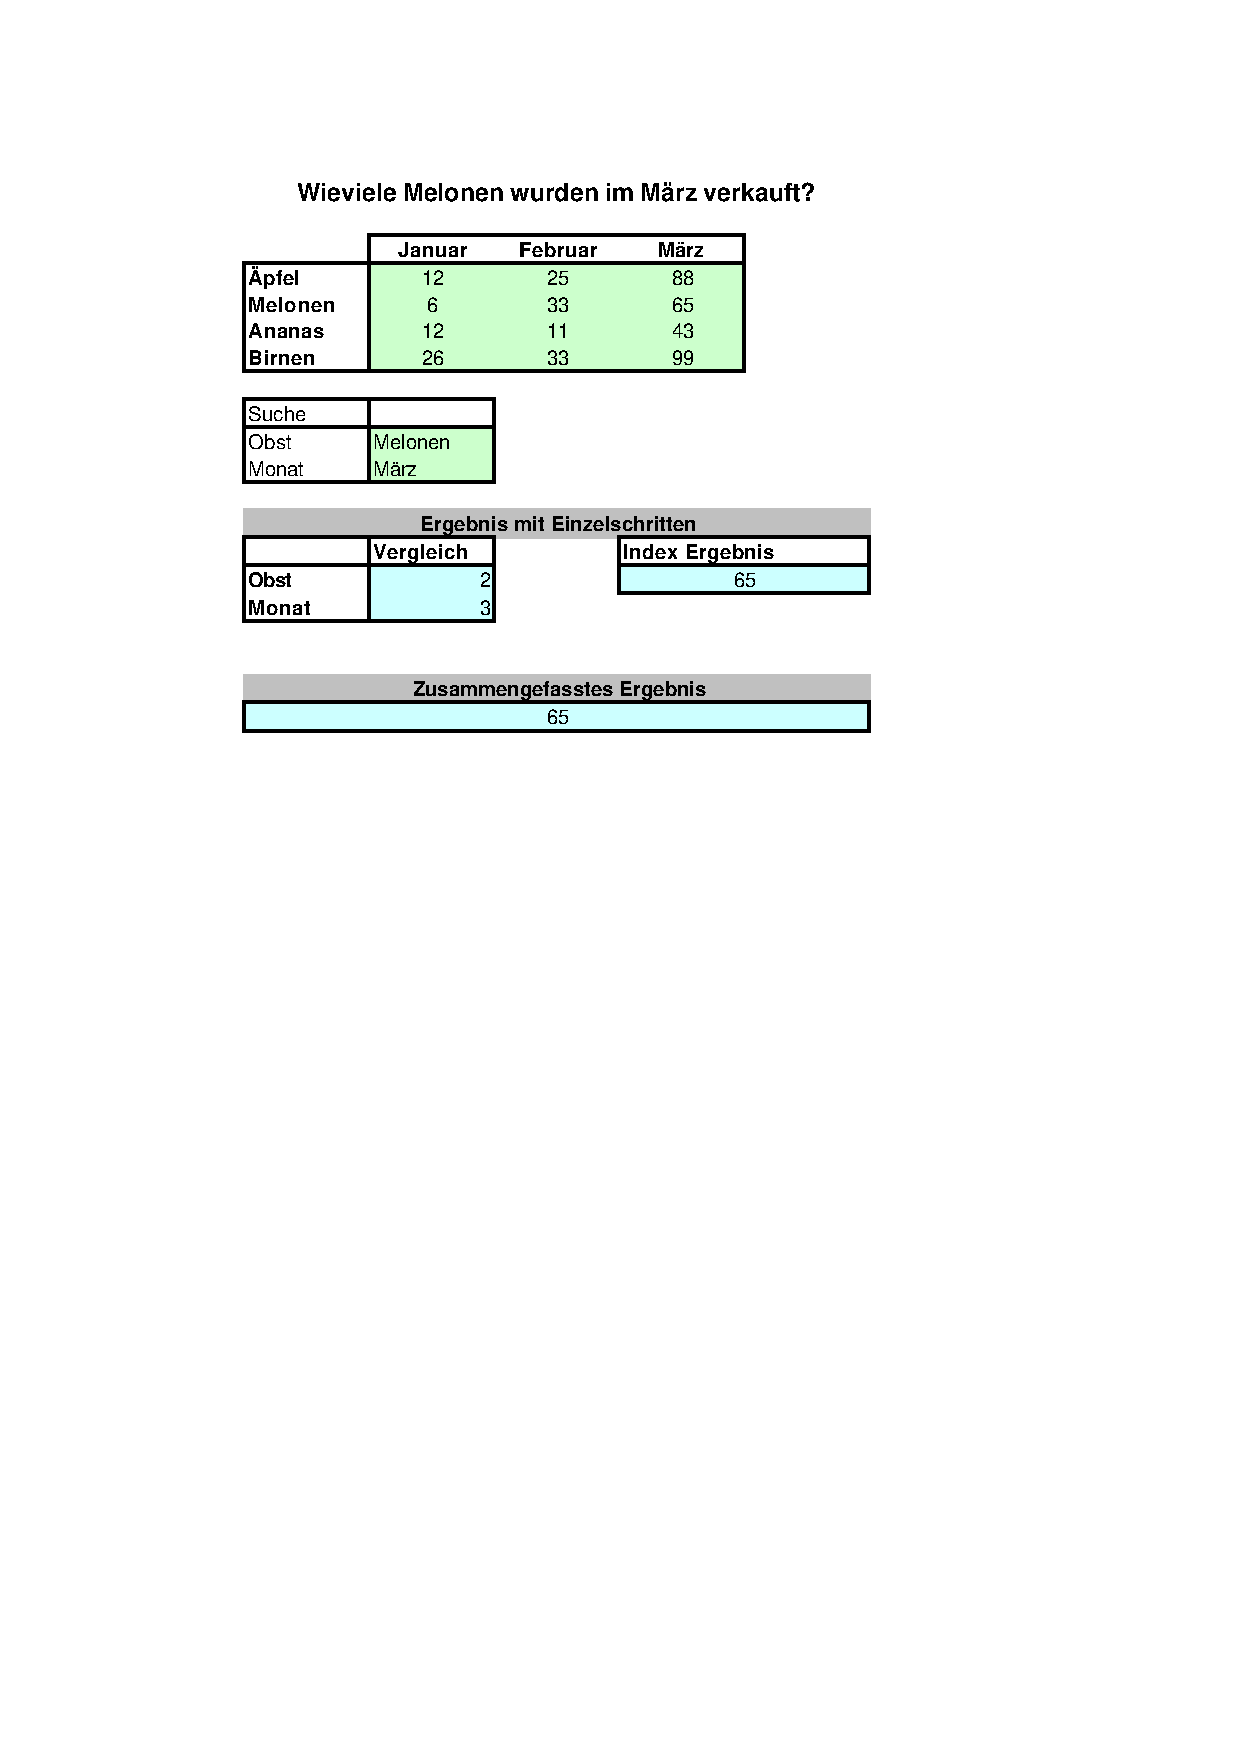
\includegraphics{images/Index_Grundbeispiel}
			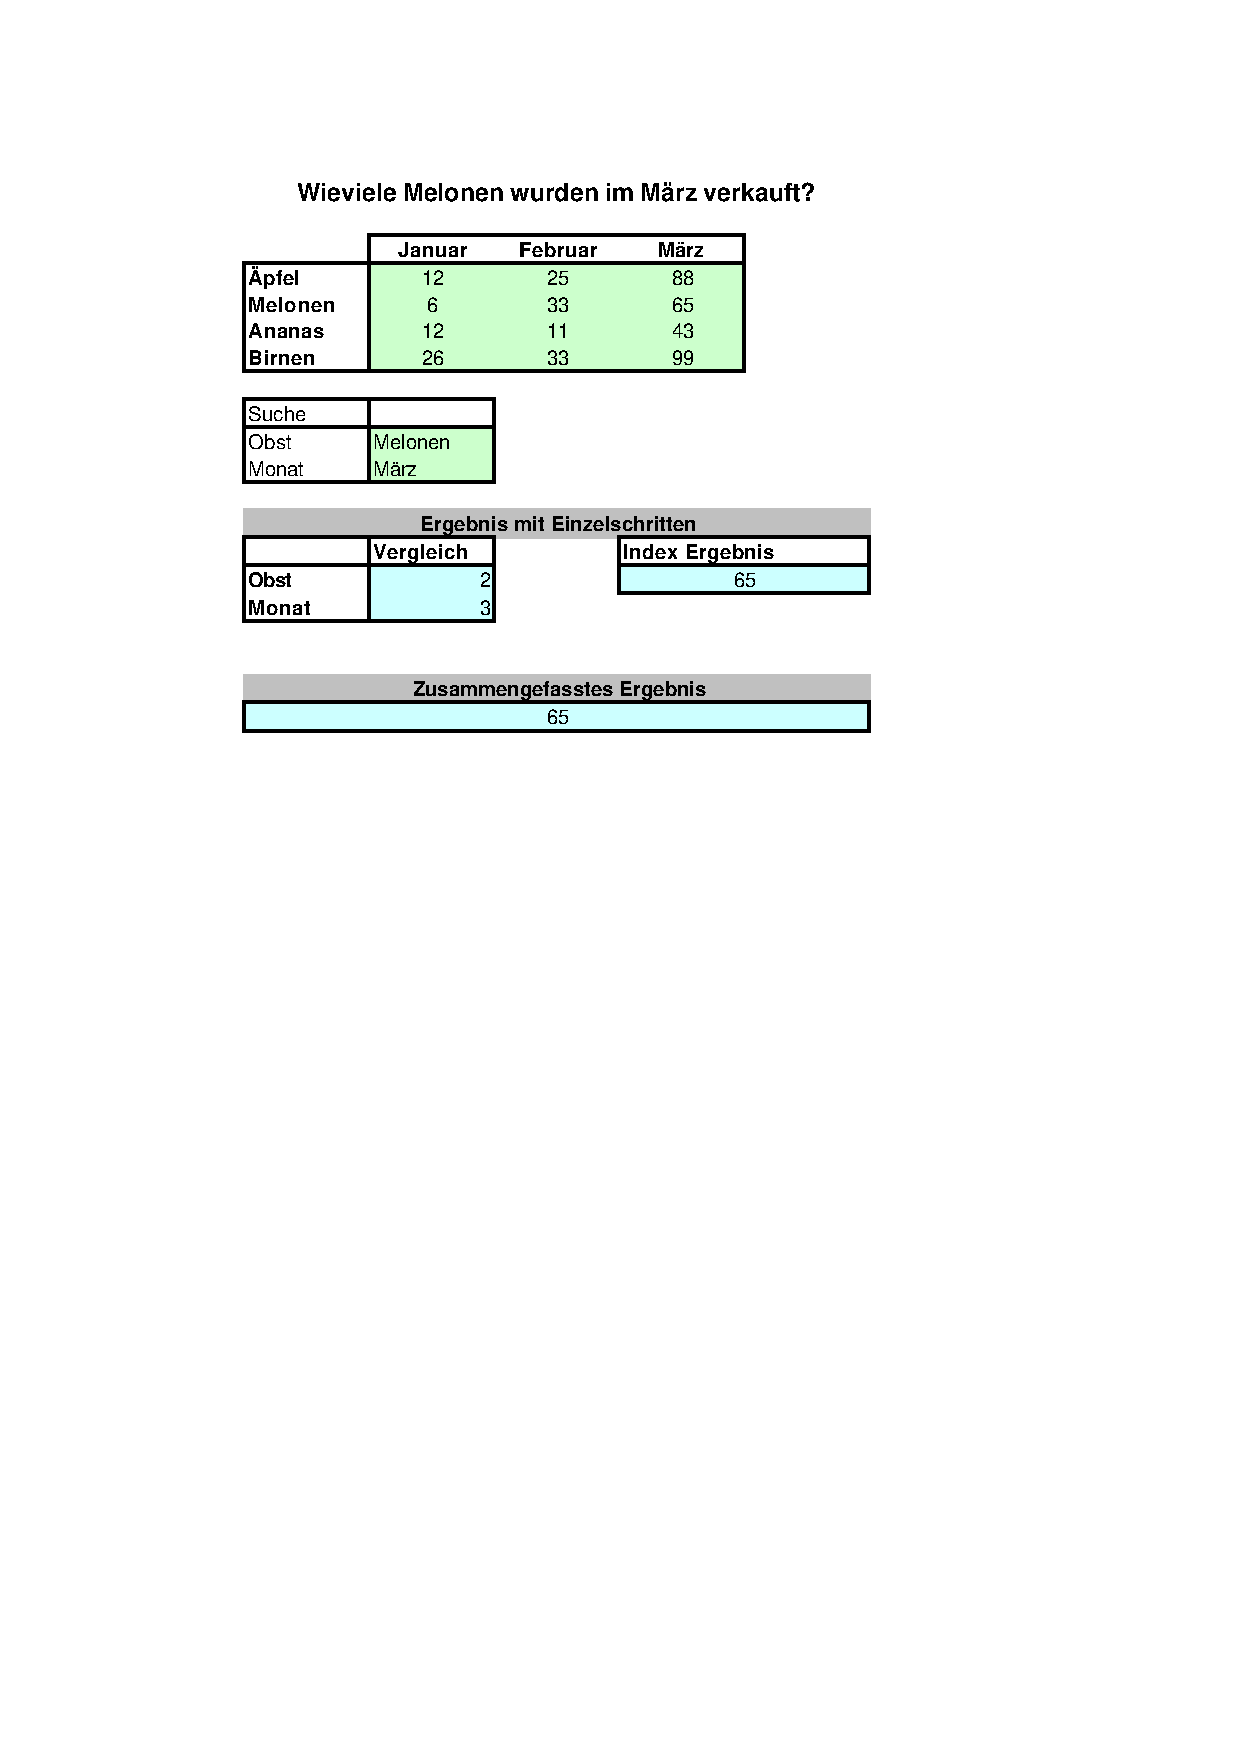
\includegraphics[scale=0.7]{images/Index_Grundbeispiel}
		\caption{Verkaufsliste des Obsthändlers}
		\label{fig:index_grundbeispiel}
	\end{figure}

Sieht man sich die Tabelle im Bereich \stmt{C5:E8} an, kann man erkennen, dass der gesuchte Wert der Schnittpunkt der Zeile 6, für die Melonen, und der Spalte E, für den Monat März, ist. Auf die Matrix bezogen ist der gesuchte Wert in der zweiten Zeile und der dritten Spalte. Die Spalten- und Reihenbezeichnung darf hier, wie bereits oben erwähnt, nicht miteinbezogen werden.


%\placefigure[middle,force]{}{\externalfigure[indexmatrix]}
	\begin{figure}[H]
		\centering
%			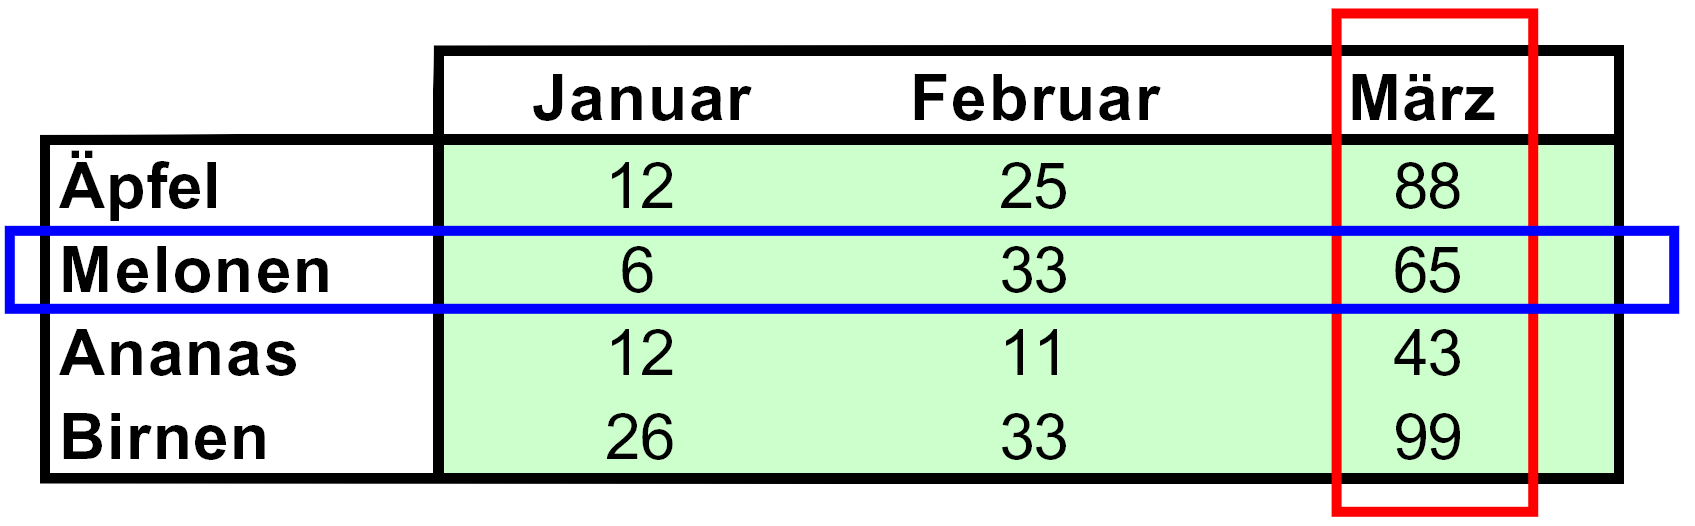
\includegraphics{images/index_matrix}
			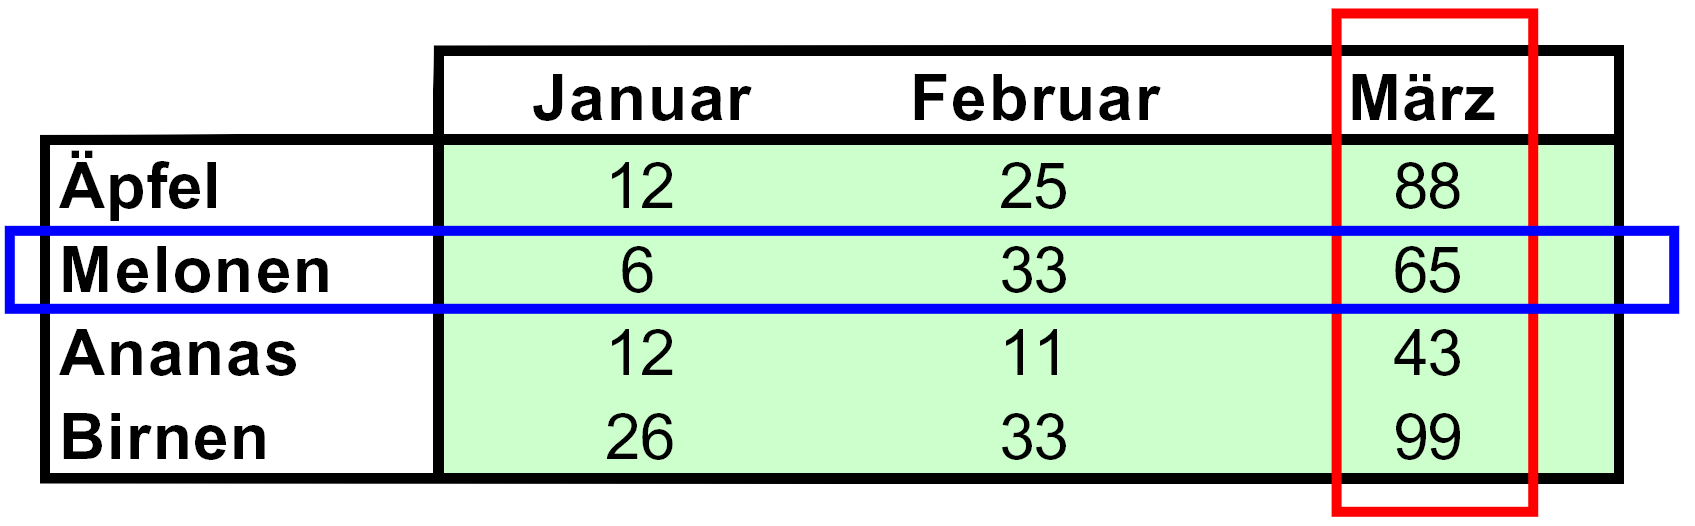
\includegraphics[scale=0.7]{images/index_matrix}
		\caption{Schnittpunkt mit dem gesuchten Wert}
		\label{fig:index_matrix}
	\end{figure}

Jetzt bleibt noch die Frage wie man die richtige Zeile und Spalte findet. Das einfachste ist, im Bereich \xlc{B5:B8} nach dem Wort Melonen und im Bereich \xlc{C4:E4} nach März zu suchen. Dafür wird die Excel Funktion \stmt{VERGLEICH} angewendet, welche in einem Suchbereich nach dem Suchkriterium gesucht. Man erhält die relative Position des gesuchten Elementes im Suchbereich.%
$$ \text{ \stmt{=VERGLEICH( \syntax{Suchkriterium}; \syntax{Suchbereich}; \syntax{Vergleichstyp})} }$$


\begin{figwindow}[0,r,{
		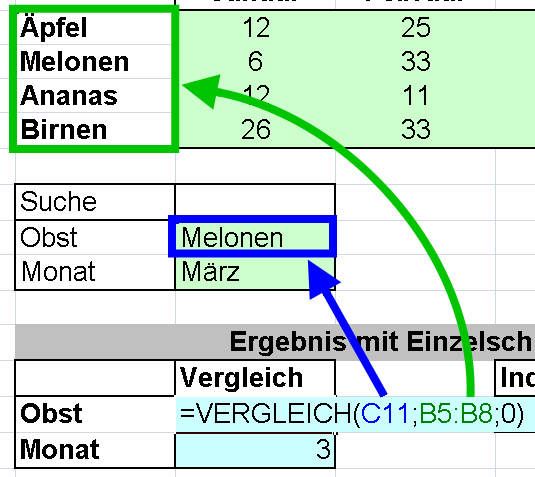
\includegraphics[width=5cm]{images/matrix_melonen}
%		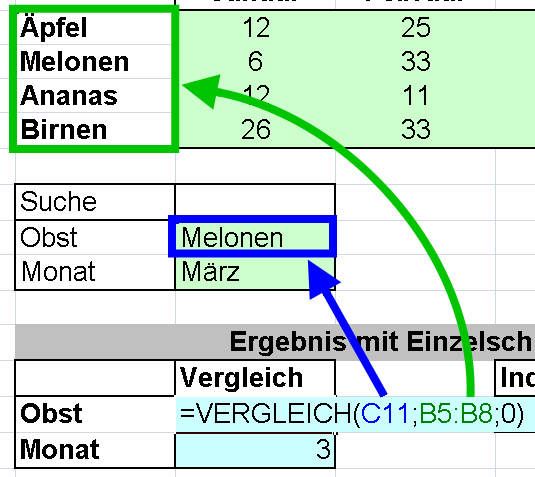
\includegraphics[scale=0.7]{images/matrix_melonen}
		\label{fig:matrixmelonen}} , {Melonen}
]
Zuerst wird in \xlc{C16} die Zeile der Matrix \xlc{B5:B8} mit dem Text Melonen ermittelt.

$ \text{\stmt{=VERGLEICH(C11; B5:B8; 0)}} $

Es wird also der Inhalt von \xlc{C11} im Bereich \xlc{B5:E8} gesucht. Der dritte Parameter der Vergleichfunktion bestimmt die Art des Vergleiches. Wenn er 0 ist, dann wird nach einer genauen Übereinstimmung gesucht. Wie zu erwarten war, erhält man den Wert 2, was nichts anderes bedeutet, dass in der zweiten Zelle des Suchbereiches der gesuchte Wert zu finden ist.%
\end{figwindow} 

\vspace{0.5cm}
\begin{figwindow}[0,r,{
		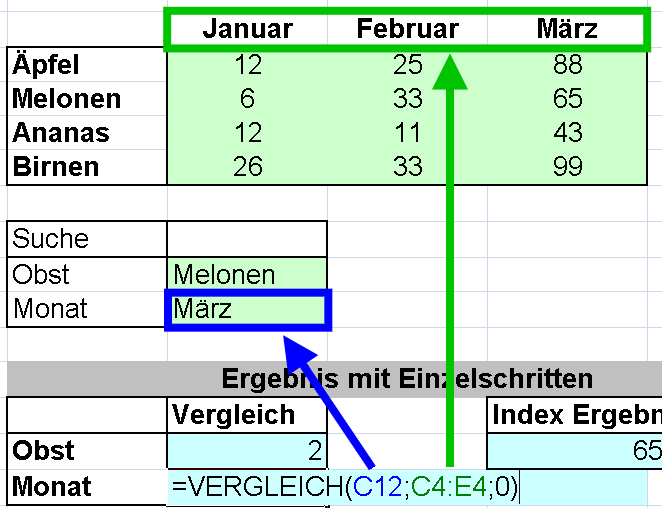
\includegraphics[width=5cm]{images/matrix_maerz}
		\label{fig:matrixmaerz	}} , {März}
]

Genauso wird nun beim Monat verfahren, dessen Spalte in  \xlc{C17} ermittelt wird.
$ \text{ {\stmt{=VERGLEICH(C12; C4:E4; 0)}}} $
%
Das Ergebnis ist, dass der Monat März in der dritten Zelle des Bereiches \xlc{C4:E4} zu finden ist.
\end{figwindow} 
\vspace{2.5cm}
%
Nachdem nun sowohl die Spalte als auch die Zeile des Datenbereiches bekannt ist, kann man mit der Funktion \stmt{INDEX} den gesuchten Wert aus der Matrix ermitteln.
%
$$ \text{\stmt{=INDEX(\syntax{Matrix}; \syntax{Zeile}; \syntax{Spalte})}} $$%
%
Überträgt man nun die ermittelte Zeile und Spalte in diese Formel, so sieht das Ergebnis so aus
%
$$ \text{\stmt{=INDEX(C5:E8; C16; C17)}} $$
%
Die Zwischenschritte werden normalerweise nicht gemacht, sondern es wird die komplette Formel in einer Zelle verwendet. Dann sieht das Ergebnis so wie in \stmt{D21} aus
%
$$ \text{\stmt{=INDEX(C5:E8;VERGLEICH(C11;B5:B8;0);VERGLEICH(C12;C4:E4;0))}} $$%
%